\documentclass[a4paper,10pt]{article}
\usepackage[utf8]{inputenc}

\usepackage{tikz}
\usepackage{bbm}
\usepackage{amsmath}

\newcommand\Shifted[2]{\Delta_{#1}(#2)}

\newcommand\SymSquare{\begin{tikzpicture}%
        \draw (0,0) -- (0,1em) -- (1em,1em) -- (1em,0) -- cycle;
\end{tikzpicture}}
\newcommand\Indicator[1]{\SymSquare(#1)}

\newcommand\SymPositiveTriangle{
\begin{tikzpicture}%
        \draw (0,0) -- (1em,0em) -- (1em,1em) -- cycle;
\end{tikzpicture}}
\newcommand\PositiveTriangle[1]{\SymPositiveTriangle(#1)}

\newcommand\SymNegativeTriangle{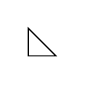
\begin{tikzpicture}%
        \draw (0,0) -- (0,1em) -- (1em,0em) -- cycle;
\end{tikzpicture}}
\newcommand\NegativeTriangle[1]{\SymNegativeTriangle(#1)}

\newcommand\SymTrapezoid{\begin{tikzpicture}%
        \draw (0,0) -- (3em) -- (2em,1em) -- (1em,1em) -- cycle;
\end{tikzpicture}}
\newcommand\Trapezoid[2]{\SymTrapezoid(#1,#2)}

\newcommand\Convolution{\star}
\newcommand\ConvolutionInt[2]{\int_{-\infty}^{\infty}#1 \mathrm{d}#2}

\title{Convolution formulas using shapes}
\author{Francois Gindraud}
\date{}

\begin{document}

\maketitle

Formulas for convolutions are very quickly unwieldy, especially if the functions being convoluted are defined by parts.
This document shows the \emph{shape} approach to convolutions: functions are decomposed into simple geometrical shapes, and convolution of the functions are defined by combining the convolutions of simple shapes.

Pros:
\begin{itemize}
    \item Manipulate only small formulas for each shape.
    \item Individual shape convolution formulas are easier to check than huge flat formulas with lots of min/max.
    \item More readable implementation of formulas into code.
    \item High level simplifications are easier to detect if some shapes cancel with others.
\end{itemize}
Cons:
\begin{itemize}
    \item Missed simplification opportunities, if the simplifications only happen between the formulas of different shapes.
    \item More verbose than the flat strategy.
\end{itemize}

\paragraph{Convolution}
Convolution is noted using the $\Convolution$ operator, with the usual definition:
\[ \left[ f \Convolution g \right](x) = \ConvolutionInt{f(x - t) g(t)}{t} \]
Convolution is commutative and associative.

\section{Combinators}

\paragraph{Time shifting}
The time shift combinator of shift $h$ moves the shape $f$ forward along the time axis by $h$.
For a shape $f$ \emph{centered} on $c$, $\Shifted{h}{f}$ is \emph{centered} on $c+h$.
\[ \Shifted{h}{f}(x) = f(x - h) \]
Time shifts combine additively:
\[ \Shifted{h}{\Shifted{h'}{f}}= \Shifted{h+h'}{f} \]
Convolution of shifted functions is the shift of convolutions:
\[
    \left[ \Shifted{h}{f} \Convolution g \right](x) =
    \ConvolutionInt{ f((x - t) - h) g(t) }{t} = 
    \left[ f \Convolution g \right](x-h) =
    \Shifted{h}{f \Convolution g}(x)
\]

\paragraph{Scaling}
The scaling combinator scales the shape $f$ by a factor $c$ on the vertical axis.
\[ \left[ c \times f \right] (x) = c \times f(x) \]
Scaling combines multiplicatively with itself, and can be swapped with time shift:
\[ c \times (c' \times f) =  (c \times c') \times f \]
\[ c \times (\Shifted{h}{f}) = \Shifted{h}{c \times f} \]
Convolution of scaled functions is a scaled convolution:
\[ (c \times f) \Convolution g = c \times (f \Convolution g) \]

\section{Basic shape definitions}

\paragraph{Indicator function}
The \emph{indicator function} of width $l$ is a rectangle of width $l$, height $1$, horizontally centered on $0$.
\begin{center}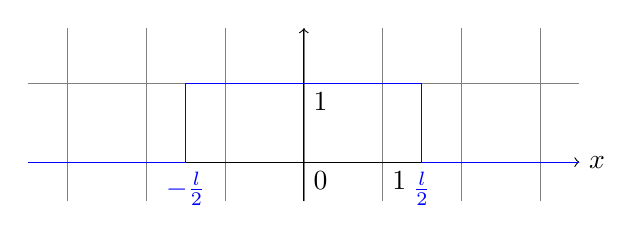
\begin{tikzpicture}
    % Grid, axis, ticks
    \draw[very thin,color=gray] (-3.5,-0.5) grid (3.5,1.7);
    \draw[->] (-3.5,0) -- (3.5,0) node[right] {$x$};
    \draw[->] (0,-0.5) -- (0,1.7);
    \node[below right] at (0,0) {$0$};
    \node[below right] at (0,1) {$1$};
    \node[below right] at (1,0) {$1$};
    % Function
    \draw[color=blue] (-3.5,0) -- (-1.5,0) -- (-1.5,1) -- (1.5,1) -- (1.5,0) -- (3.5,0);
    \node[below,color=blue] at (-1.5,0) {$-\frac{l}{2}$};
    \node[below,color=blue] at (1.5,0) {$\frac{l}{2}$};
\end{tikzpicture}\end{center}
\[
    \Indicator{l}(x) =
    \mathbbm{1}_{\left[ -\frac{l}{2}, \frac{l}{2} \right]}(x) =
    \begin{cases}
        1 & x \in \left[ -\frac{l}{2}, \frac{l}{2} \right] \\
        0 & \text{otherwise}
    \end{cases}
\]
The function is symmetric:
\[ \Indicator{l}(-x) = \Indicator{l}(x) \]

\paragraph{Positive triangle}
The \emph{positive triangle} of side $c$ is a triangle formed by coordinates $\{ (0,0), (c, 0), (c,c) \}$:
\begin{center}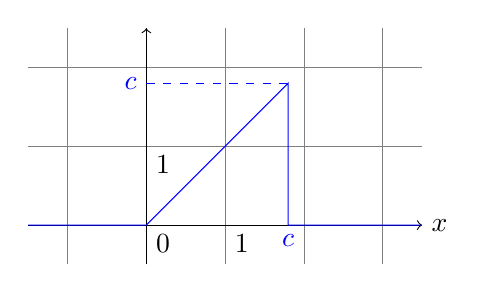
\begin{tikzpicture}
    % Grid, axis, ticks
    \draw[very thin,color=gray] (-1.5,-0.5) grid (3.5,2.5);
    \draw[->] (-1.5,0) -- (3.5,0) node[right] {$x$};
    \draw[->] (0,-0.5) -- (0,2.5);
    \node[below right] at (0,0) {$0$};
    \node[below right] at (0,1) {$1$};
    \node[below right] at (1,0) {$1$};
    % Function
    \draw[color=blue] (-1.5,0) -- (0,0) -- (1.8,1.8) -- (1.8,0) -- (3.5,0);
    \draw[dashed,color=blue] (0,1.8) -- (1.8,1.8);
    \node[left,color=blue] at (0,1.8) {$c$};
    \node[below,color=blue] at (1.8,0) {$c$};
\end{tikzpicture}\end{center}
\[
    \PositiveTriangle{c}(x) = \begin{cases}
        x & x \in \left[ 0, c \right] \\
        0 & \text{otherwise}
    \end{cases}
\]

\paragraph{Negative triangle}
The \emph{negative triangle} of side $c$ is a triangle formed by coordinates $\{ (0,0), (-c, 0), (-c,c) \}$:
\begin{center}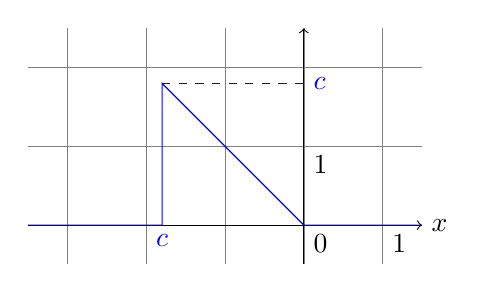
\begin{tikzpicture}
    % Grid, axis, ticks
    \draw[very thin,color=gray] (-3.5,-0.5) grid (1.5,2.5);
    \draw[->] (-3.5,0) -- (1.5,0) node[right] {$x$};
    \draw[->] (0,-0.5) -- (0,2.5);
    \node[below right] at (0,0) {$0$};
    \node[below right] at (0,1) {$1$};
    \node[below right] at (1,0) {$1$};
    % Function
    \draw[color=blue] (-3.5,0) -- (-1.8,0) -- (-1.8,1.8) -- (0,0) -- (1.5,0);
    \draw[dashed,color=blue] (-1.8,1.8) -- (0,1.8);
    \node[right,color=blue] at (0,1.8) {$c$};
    \node[below,color=blue] at (-1.8,0) {$c$};
\end{tikzpicture}\end{center}
\[
    \NegativeTriangle{c}(x) = \begin{cases}
        -x & x \in \left[ -c, 0 \right] \\
        0 & \text{otherwise}
    \end{cases}
\]
A reversed negative triangle is a positive triangle:
\[ \NegativeTriangle{c}(-x) = \PositiveTriangle{c}(x) \]

\paragraph{Trapezoid}
A \emph{trapezoid} of height $h$ and central block width $b$ is formed by a central rectangle of size $(b,h)$ centered on $0$, and flanked by triangles of side size $h$:

\begin{center}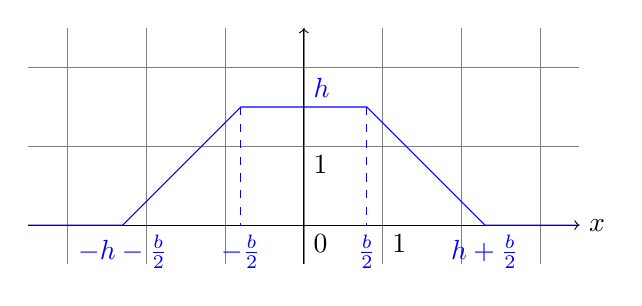
\begin{tikzpicture}
    % Grid, axis, ticks
    \draw[very thin,color=gray] (-3.5,-0.5) grid (3.5,2.5);
    \draw[->] (-3.5,0) -- (3.5,0) node[right] {$x$};
    \draw[->] (0,-0.5) -- (0,2.5);
    \node[below right] at (0,0) {$0$};
    \node[below right] at (0,1) {$1$};
    \node[below right] at (1,0) {$1$};
    % Function
    \draw[color=blue] (-3.5,0) -- (-2.3,0) -- (-0.8,1.5) -- (0.8,1.5) -- (2.3,0) -- (3.5,0);
    \node[above right,color=blue] at (0,1.5) {$h$};
    \draw[dashed,color=blue] (-0.8,1.5) -- (-0.8,0) node[below] {$-\frac{b}{2}$};
    \draw[dashed,color=blue] (0.8,1.5) -- (0.8,0) node[below] {$\frac{b}{2}$};
    \node[below,color=blue] at (-2.3,0) {$-h-\frac{b}{2}$};
    \node[below,color=blue] at (2.3,0) {$h+\frac{b}{2}$};
\end{tikzpicture}\end{center}
%TODO formula
%TODO decomposition
%TODO convolution of square,square, +link to proof

\section{Convolution shapes}

\section{Proofs}

\end{document}
